
% !TeX root = ./report.tex
\chapter{Background}
Vulnerabilities in software can lead to catastrophic consequences when manipulated by attackers. In an open-source cryptographic software library (OpenSSL) used by an estimated two-thirds of web servers \cite{heartbleed} a security flaw called Heartbleed was discovered. Secure secrets such as financial data, encryption keys, or anything else stored in the server's memory could be leaked. Normally, one would send a Heartbeat request with a text string payload and the length of the payload. For example, a message of ``hello'' could be sent with the length of the message, 5. However, due to a improper input validation (buffer over-read), one could send a length longer that the string they actually sent. This would cause the server to respond with the original message and anything that was in the allocated memory at the time, including any potentially sensitive information. An example of this is shown in figure \ref{fig:heartbleed} \cite{heartbleedimg}.

\begin{figure}
    \centering
    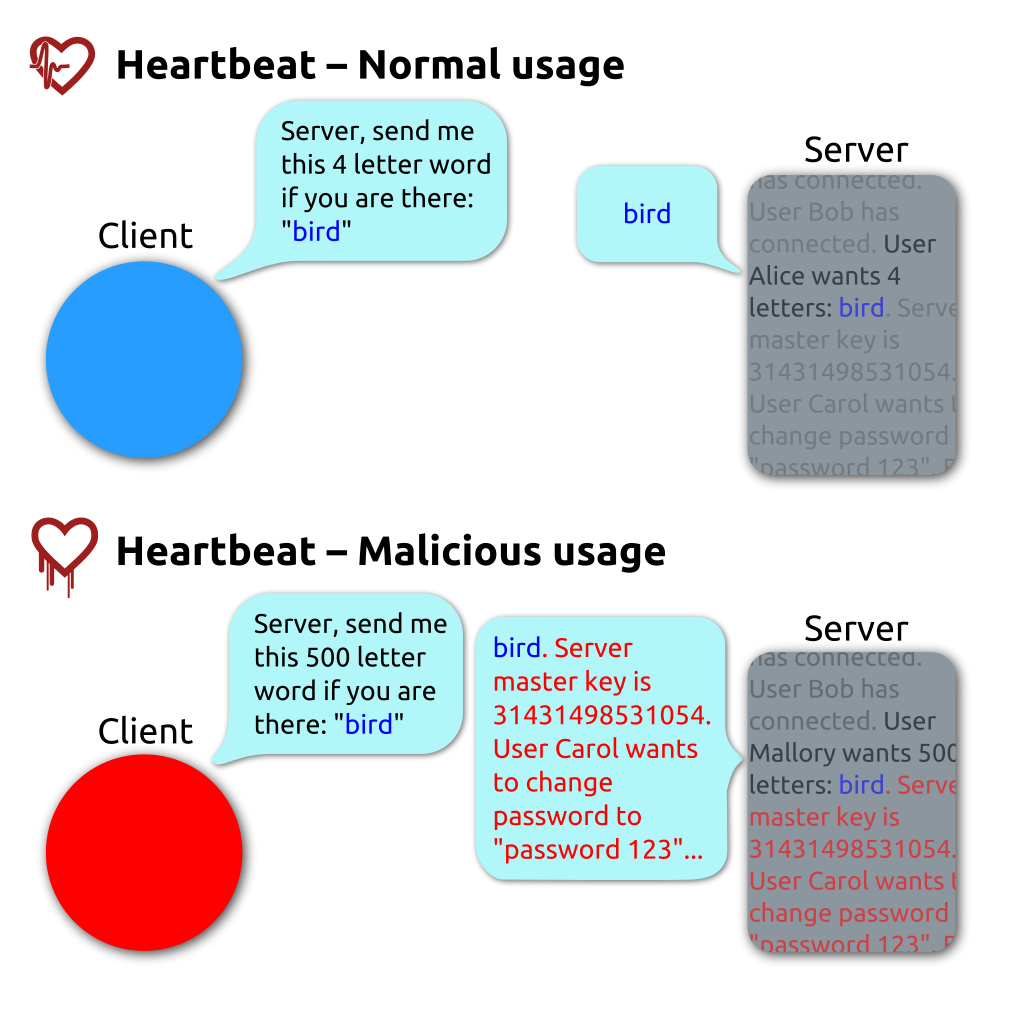
\includegraphics[width=0.5\linewidth]{heartbleed.png}
    \caption{The Heartbleed bug. \cite{heartbleedimg}}
    \label{fig:heartbleed}
\end{figure}

Heartbleed was one of the most dangerous security bugs ever, and calls for major reflection by everyone in industry and research \cite{balliu2014logics}.

\section{Information Security}

Computer security is defined as a preservation of \textbf{integrity}, \textbf{availability} and \textbf{confidentiality} of information, and extends to include not only software but hardware, firmware, information, data and telecommunications \cite{guttman1995introduction}.
Confidentiality requires that data is not available to unauthorised users, and that individuals can control what information can be collected and disclosed to others. Data integrity requires that only authorised sources can modify data, and that the system can perform tasks without interference from outside sources. Finally, availability of a system requires that service is not denied to authorised users. Together, these principles create the CIA triad \cite{stallings2012computer}. To enforce a secure system, all three principles must be upheld.

Modern programs are becoming increasingly complex with potential for networking, multi-threading and storage permissions and more. As such, security mechanisms must be put in place to verify and enforce the information security requirements. The adequacy of a security mechanism depends on the adversary model. The adversary model is a formal definition of the attacker and their abilities in a system, and defines who we are protecting against \cite{do2019role}. Ideally we would like to design a system to protect against the strongest adversary or attacker, however, this is often not required or even possible. Instead, we must consider the security policy, security mechanism and strongest adversary model to make a system secure \cite{balliu2014logics}.

Standard security processes that handle access control such as a firewall or antivirus software can fail as they do not constrain where information is allowed to flow, meaning that once access is granted it can propagate to insecure processes where it can be accessed by attackers. Where a large system is being used, it is often the case that not all components of the codebase can be trusted, often containing potentially malicious code \cite{sabelfeld2003language}. Take for example your modern-day web project. Where a package manager such as Node Package Manager (npm) could be used to utilise open-source packages to speed up development progress, it could also inadvertently introduce security vulnerabilities. Rewriting all packages used to ensure security would be time-consuming and expensive and is not a viable option. Instead, controlling where information can flow and preventing secure data from flowing into untrusted sources or packages can maintain confidentiality of a system.

One may suggest runtime monitoring the flow of data to prevent leakage of secure data. Aside from the obvious computational and memory overhead, this method can have its own issues. Although it can detect an \textit{explicit} flow of data from a secure variable to a public variable, it is unable to detect \textit{implicit} data flow, where the state of secure data can be inferred from the state of public data or a public variable \cite{denning1977certification}. Take for example figure \ref{fig:implicit}. In this example, a public, readable variable is initially set to the value of 1. There is also a secret variable which may contain a key, password or some other secret that must be kept secure from any attackers. Depending on the value of the secret variable an attacker can infer information about this variable depending on whether the value of the public variable is updated to a value of 0. Assuming that the inner workings of the system is known by the attacker, information about the secret variable can be leaked \textit{implicitly} and inferred by the state of public variables.

\begin{figure}
    \begin{lstlisting}
secret := 0xC0DE mod 2
public := 1
if secret = 1
    public := 0
        \end{lstlisting}
    \caption{Implicit flow of data to a public variable}
    \label{fig:implicit}
\end{figure}

Security concerns do not only exist at the application level. In a huge codebase such as an OS, different low-level bugs can be exploited to gain access to data, such as by using buffer overflows to inject viruses or trojans \cite{agten2012recent}.

\section{Information Flow Control}
As seen by the issues that can be introduced via implicit and explicit flow of data, there is room to improve on the existing techniques imposed by current security measures. To protect confidentiality, secure or sensitive information must be prevented from flowing into public on insecure variables. Additionally, to protect integrity, untrusted data from public sources must be prevented from flowing into secure or trusted destinations \cite{balliu2014logics}. An information flow security policy can be introduced to classify or label data, or more formally, a set of \textit{security levels} to which each object is bound by across a multi-level security lattice \cite{denning1976lattice}. In this thesis, we will focus primarily on preserving confidentiality.

Many security levels can be identified to classify different classes of objects, however, for now we will consider two security levels: high and low. Data labelled as high signifies that the data is secret, and low data is classified as non-sensitive data, such that it does not need to be protected from an attacker or adversary. Variables that can hold data in a program can additionally be classified as high or low as a \textit{security classification}. A variable's security classification shows the highest classification of data it can safely contain \cite{winter2020information}. A high variable can hold both high and low data, whereas a low variable which is visible to an attacker can only safely hold low data. As mentioned previously, confidentiality must be upheld by preventing high or secret data from flowing to low or public variables where an attacker can observe it. The permitted flow of data can be observed in \ref{fig:flow}. Note that high data is not allowed to flow into low variables.

\begin{figure}
    \centering
    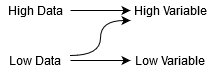
\includegraphics[width=0.5\linewidth]{flow.png}
    \caption{Permitted flow of data}
    \label{fig:flow}
\end{figure}

\section{Information Flow Security in Concurrency}
Controlling the flow of information is a difficult problem, however, this is only exacerbated in concurrent programs, which are a well known source of security issues \cite{mantel2014noninterference}\cite{smith2019value}\cite{vaughan2012secure}. Research has been conducted into concurrent programs to explore ways the security of concurrent programs can be verified. Mantel et al. \cite{mantel2011assumptions} introduced the concept of assumption and guarantee conditions, where assumptions are made about how concurrent threads access shared memory and guarantees are made about how an individual thread access shared memory that other threads may rely upon. Each thread can be observed individually using assumptions over the environment behaviour of other threads that can be then used to prove a guarantee about that individual thread. As two concurrent threads can interleave their steps and behaviour, there is a lot of complexity and possibilities for the overall behaviour. This concept of assumptions (or rely) and guarantee conditions can reduce the complexity of understanding interleaving behaviour in threads and assist in verifying the correctness of information flow security in concurrency. However, this approach is limited in the types of assumptions and guarantees it supports. Building on this, Murray et al. \cite{ernst2019seccsl} \cite{murray2018covern} provide information flow logic on how to handle dynamic, value-dependent security levels in concurrent programs. In this case, the security level of a particular variable may depend on one or more other variables in the program. As such, the variable's security level can change as the state of the program changes. This logic is essential where the security level of data depends on its source. However, this approach is not sufficient when analysing non-blocking programs. The approach relies heavily on locks which block particular threads from executing. This in turn leads to slower processing due to blocked threads \cite{prakash1991non}.

To overcome information flow security in non-blocking concurrent threads, Winter et al. \cite{winter2020information} explores verifying security properties such as non-interference through the use of general rely/guarantee conditions using backwards, weakest precondition reasoning. Such an analysis would additionally handle implicit flows as shown in figure \ref{fig:flow}. Ideally a tool could be created to verify security policies required for sensitive processes. Users of this system could provide rely/guarantee conditions for each thread as well as security levels for data and variables i.e. high or low data and variables. Working backwards through the execution of the program, violations of the security policy will be detected. Detected violations could be due to an incorrect assumption of the rely and guarantee conditions or a failure to uphold the security policy. This thesis will focus on the compilation stage of this tool.

\section{Compilers and Security}
\label{sec:compilersSecurity}
Compilers are well known to be a weak link between source code and the hardware executing it. Source code that has been verified to provide a security guarantee, potentially using formal techniques, may not hold those security guarantees when being executed. This is caused by compiler optimisations that may be technically correct, however, a compiler has no notion of timing behaviour or on the expected state of memory after executing a statement \cite{d2015correctness}. This problem is known as the \textit{correctness security gap}. One example of the correctness security gap is caused by an optimisation called dead store elimination. Figure \ref{fig:deadstore} was derived from CWE-14 \cite{cwe14} and CWE-733 \cite{cwe733} and used by D'Silva et al. \cite{d2015correctness}. Here a secret key was retrieved and stored in a local variable to perform some work. After completing the work, and to prevent sensitive data from flowing into untrusted sources, the key is wiped from memory by assigning it the value 0x0.

\begin{figure}
    \begin{lstlisting}
crypt() {
    key := 0xC0DE // Read key
    ... // Work with the key
    key := 0x0 // Clear memory
}
    \end{lstlisting}
    \caption{Implicit flow of data to a public variable \cite{d2015correctness}}
    \label{fig:deadstore}
\end{figure}

From the perspective of the source code, a programmer would expect the sensitive data from key to be scrubbed after exiting the function. However, key is a variable local to the function. As key is not read after exiting the function, the statement that assigns key to a value of 0x0 will be removed as part of dead store elimination. This results in lingering memory that could be exploited by an attacker. In GCC, with compiler optimisations on, dead store elimination is performed by default \cite{gccoptimise}. Additionally, dead store elimination has been proven to be functionally correct \cite{benton2004simple}\cite{leroy2006formal}.

% TODO: Discuss what other compiler optimisations can cause the correctness security gap

This leads to the question, \textit{what security guarantees in source code are being violated by compiler optimisations?} Although one could analyse each individual compiler optimisation to check for potential security violations in source code, defensively programming against the compiler can be counter-initiative. Additionally, compilers are getting better at optimising away tricks programmers write to work against the compiler, and thus is not a future-proof solution \cite{simon2018you}. One might also suggest turning compiler optimisations off, however, this leads to slower code. In a concurrent system where execution time is critical, turning compiler optimisations off is not a viable option. Instead an alternative solution is to perform a static analysis on binary or assembly for security violations. As compilation has already been executed, such analysis would reveal security guarantee violations that result due to compiler optimisations.

\section{Annotations}
This project can take two routes; the proposed solution will be required to preserve annotations to either binary or assembly. For either route, annotations used to guide a static security analysis will need to be provided by the user in the C programs they write. The annotations will then be required to propagate down to compiled forms, i.e. binary or assembly. From here, a static analysis can be conducted as described by Winter et al. \cite{winter2020information}. Ideally these annotations can be propagated through with little to no modification of the C Compiler being used as to reduce complexity and increase modularity and reusability of such a a tool. However, it is unclear as to whether passing annotations down without modifying the compiler is currently possible. In this thesis, this issue will be explored.

Running a static analysis on a binary can be difficult due to the low level nature of a binary file. As such, to sufficiently perform such an analysis, the binary would be required to be decompiled to a higher-level form, such as an assembly file. From here a static analysis could be conducted. The alternative approach would be to perform the analysis directly on the compiled assembly output files rather than reducing these to binary. Currently, it is unclear as to what compiler optimisations are made when reducing an assembly file to binary, and will be explored further throughout the lifetime of this thesis. The flow of information can be viewed in Figure \ref{fig:analysis}, where formats a static analysis can be performed are outlined in a dashed line. In GCC, ``temporary'' intermediate files can be stored using the flag \textit{save-temps} \cite{gccdevoptions}. These stored files can then be used for analysis.


\begin{figure}
    \centering
    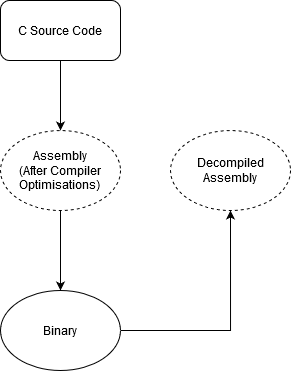
\includegraphics[width=0.5\linewidth]{compilation.png}
    \caption{The static analysis options after compilation.}
    \label{fig:analysis}
\end{figure}

% TODO: Include figure of this problem

% TODO: Symbol table.

\section{Related Work}
In safety-critical real-time software such as flight control systems, it is required to analyse the \textit{Worst Case Execution Time} (WCET). This kind of analysis can be conducted using static analysis tools to estimate safe upper bounds. In the case of AbsInt's aiT tool this analysis is conducted alongside compiler annotations to assist where loop bounds cannot be computed statically. In these cases, the user can provide annotations to guide the analysis tools \cite{schommer2018embedded}. This tool builds on an existing annotation mechanism that exist in CompCert, a C compiler that has been formally verified for use in life-critical and mission-critical software \cite{compcert}\cite{leroy2016compcert}. CompCert annotations are not limited to WCET analysis. A general mechanism for attaching free-form annotations that propagate through to assembly files can be achieved with CompCert. This approach is able to reliably transmit compiler annotations through to binary through method calls. These annotations do not use external annotation tools to transmit through compilation and the linked executable. CompCert prints annotation strings as a comment in the generated assembly code, and an additional tool is used to parse these comments and generate annotations. However, due to its treatment as an external function, annotations cannot be placed at the top level of a compilation unit, unlike a variable declaration. Compiler optimisations can additionally cause further issues when trying to preserve annotations through compilation. If dead code is eliminated, annotations associated with that code can be lost as well. Extra care needs to be taken to avoid these optimisations destroying links between properties and the code they refer to during such transformations.

\label{sec:relatedWorkCompCert}
% TODO: Include further documentation on how to use Compiler \& inline assembly
% https://compcert.org/man/manual006.html#sec112

A similar approach to CompCert is used by The ENTRA (Whole-Systems ENergy TRAnsparency). As part of providing a common assertion language, pragmas are used to propagate information through to comments in the assembler files. Information is retained in LLVM IR and ISA representations. However, these annotations are not stored in the final binary and thus comments must be extracted from assembler files \cite{eder2013common}.

Vu et al. \cite{vu2020secure} explore capturing and propagating properties from the source code level though though lowering passes and intermediate representations. Their goal was to maintain these properties to binary through aggressive compiler optimisations. As compilers only care about functional correctness, they have no notion of the link between properties and the code it refers to. Thus, there is no way to constrain transformations to preserve this link or to update these properties after the transformation. As such, they approached the problem to create a generic solution, modifying a LLVM compiler with virtually no optimisation changes. This was done by creating a library in LLVM. The properties were stored in strings, and these strings were parsed to build a list of observed variables and memory location. A LLVM pass was inserted to store all these properties in metadata. After each optimisation pass, a verification pass was inserted to check the presence of metadata representing the properties, variables amd memory locations. If an optimisation pass had cased the verification to fail the programmer would then be notified, to which they could annotate differently or disable the optimisation.
